\documentclass[border=5pt]{standalone}
\usepackage{tikz}
\usetikzlibrary{positioning, arrows.meta, calc}
\usepackage{amsmath}

\newcommand{\Snbr}{S_{\text{nbr}}}

\begin{document}
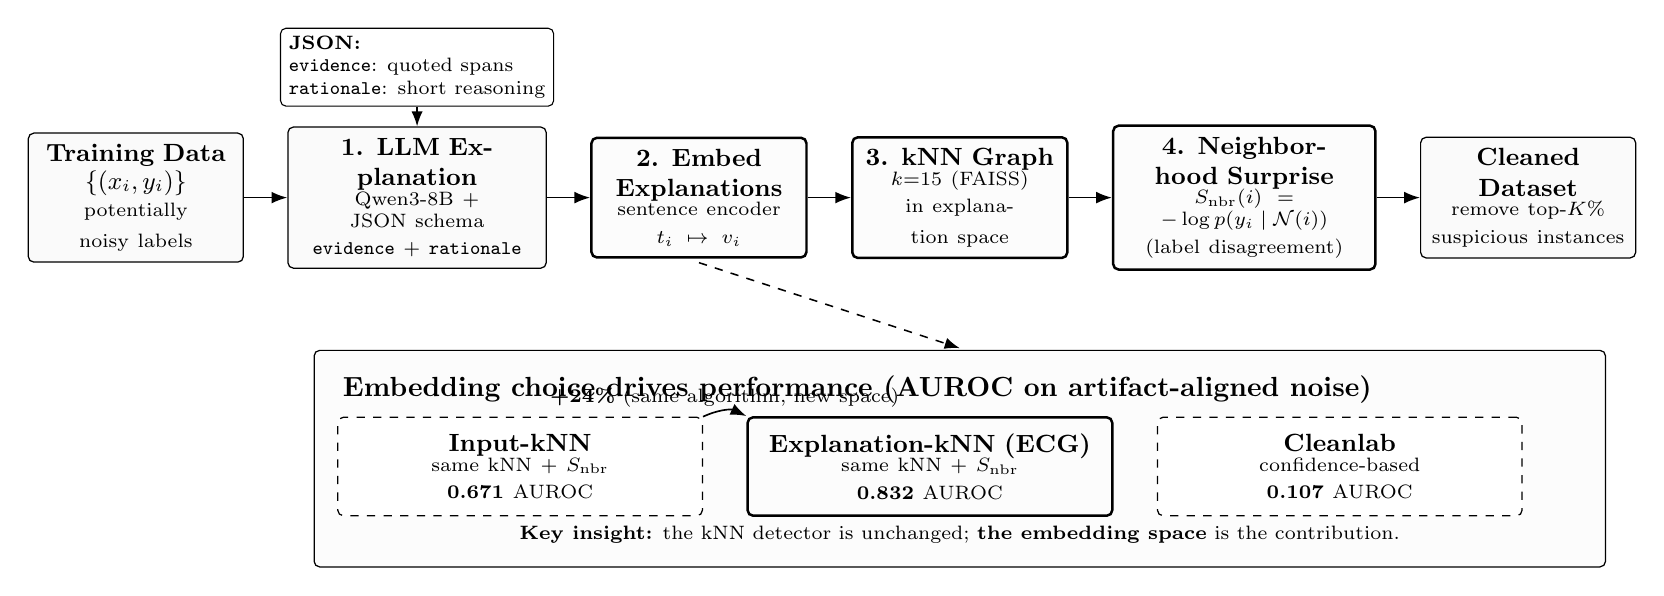
\begin{tikzpicture}[
  font=\small,
  node distance=0.55cm,
  >=Latex
]
% -------------------- Styles --------------------
\tikzset{
  block/.style={
    draw, rounded corners=2pt, line width=0.45pt,
    fill=black!2,
    align=center, inner sep=4pt,
    text width=2.45cm, minimum height=1.25cm
  },
  blockWide/.style={
    block, text width=3.00cm
  },
  focus/.style={
    block, line width=0.9pt, fill=black!1
  },
  baseline/.style={
    block, dashed, fill=white
  },
  arrow/.style={-Latex, line width=0.6pt},
  dArrow/.style={-Latex, dashed, line width=0.55pt},
  panel/.style={
    draw, rounded corners=2pt, line width=0.45pt,
    fill=black!1, inner sep=6pt
  }
}

% -------------------- Main pipeline (top row) --------------------
\node[block] (data) {
  \textbf{Training Data}\\[-1pt]
  $\{(x_i, y_i)\}$\\[-1pt]
  \scriptsize potentially noisy labels
};

\node[blockWide, right=of data] (llm) {
  \textbf{1. LLM Explanation}\\[-1pt]
  \scriptsize Qwen3-8B + JSON schema\\[-1pt]
  \scriptsize \texttt{evidence} + \texttt{rationale}
};

\node[focus, right=of llm] (embed) {
  \textbf{2. Embed Explanations}\\[-1pt]
  \scriptsize sentence encoder\\[-1pt]
  \scriptsize $t_i \mapsto v_i$
};

\node[focus, right=of embed] (knn) {
  \textbf{3. kNN Graph}\\[-1pt]
  \scriptsize $k{=}15$ (FAISS)\\[-1pt]
  \scriptsize in explanation space
};

\node[focus, right=of knn, text width=3.05cm] (snbr) {
  \textbf{4. Neighborhood Surprise}\\[-1pt]
  \scriptsize $\Snbr(i) = -\log p\!\left(y_i \mid \mathcal{N}(i)\right)$\\[-1pt]
  \scriptsize (label disagreement)
};

\node[block, right=of snbr] (out) {
  \textbf{Cleaned Dataset}\\[-1pt]
  \scriptsize remove top-$K\%$\\[-1pt]
  \scriptsize suspicious instances
};

\draw[arrow] (data) -- (llm);
\draw[arrow] (llm) -- (embed);
\draw[arrow] (embed) -- (knn);
\draw[arrow] (knn) -- (snbr);
\draw[arrow] (snbr) -- (out);

% Small callout: structured explanation fields
\node[draw, rounded corners=2pt, line width=0.4pt, fill=white,
      align=left, inner sep=3pt, font=\scriptsize,
      above=0.25cm of llm, anchor=south] (json) {
  \textbf{JSON:}\\
  \texttt{evidence}: quoted spans\\
  \texttt{rationale}: short reasoning
};
\draw[dArrow] (json.south) -- (llm.north);

% -------------------- Comparison panel (bottom) --------------------
\node[panel, below=1.15cm of knn, minimum width=16.4cm, minimum height=2.75cm, anchor=north] (comp) {};

\node[font=\bfseries, anchor=north west] at ($(comp.north west)+(0.25cm,-0.20cm)$) {Embedding choice drives performance (AUROC on artifact-aligned noise)};

\node[baseline, text width=4.35cm, minimum height=1.25cm, anchor=north west]
  (inputknn) at ($(comp.north west)+(0.30cm,-0.85cm)$) {
  \textbf{Input-kNN}\\[-1pt]
  \scriptsize same kNN + $\Snbr$\\[-1pt]
  \textbf{0.671} AUROC
};

\node[focus, text width=4.35cm, minimum height=1.25cm, right=0.55cm of inputknn]
  (expknn) {
  \textbf{Explanation-kNN (ECG)}\\[-1pt]
  \scriptsize same kNN + $\Snbr$\\[-1pt]
  \textbf{0.832} AUROC
};

\node[baseline, text width=4.35cm, minimum height=1.25cm, right=0.55cm of expknn]
  (cleanlab) {
  \textbf{Cleanlab}\\[-1pt]
  \scriptsize confidence-based\\[-1pt]
  \textbf{0.107} AUROC
};

% +24% annotation between Input-kNN and Explanation-kNN
\draw[arrow] (inputknn.north east) to[out=25, in=155]
  node[above, font=\scriptsize, inner sep=1pt] {\textbf{+24\%} (same algorithm, new space)}
  (expknn.north west);

% Panel footer message
\node[font=\scriptsize, anchor=south] at ($(comp.south)+(0,0.18cm)$) {
  \textbf{Key insight:} the kNN detector is unchanged; \textbf{the embedding space} is the contribution.
};

% Light connector from pipeline to panel
\draw[dArrow] ($(embed.south)+(0,-0.05cm)$) -- ($(comp.north)+(0,0.02cm)$);

\end{tikzpicture}
\end{document}

